\documentclass[11pt]{article}
\usepackage{latexsym}
\usepackage{amssymb,amsthm,amsmath}
\usepackage{mathrsfs}
\usepackage[pdftex]{graphicx}
\usepackage{tikz}
\usepackage{pbox}
\usepackage{indentfirst}
\usetikzlibrary{intersections, calc}
\usepackage[margin=1in]{geometry}
\usepackage{listings}

\definecolor{dkgreen}{rgb}{0,0.6,0}
\definecolor{gray}{rgb}{0.5,0.5,0.5}
\definecolor{mauve}{rgb}{0.58,0,0.82}

\lstset{frame=tb,
  language=Python,
  aboveskip=3mm,
  belowskip=3mm,
  showstringspaces=false,
  columns=flexible,
  basicstyle={\small\ttfamily},
  numbers=none,
  numberstyle=\tiny\color{gray},
  keywordstyle=\color{blue},
  commentstyle=\color{dkgreen},
  stringstyle=\color{mauve},
  breaklines=true,
  breakatwhitespace=true,
  tabsize=3
}

\graphicspath{ {figures/} }

\author{{\bf Testing, Testing, 1, 2, 4} \medskip \\ Neil Chainani, Avery Faller, Ed Weng}
\title{CS 181: Machine Learning --- Practical 3}
\date{Friday, April 8, 2016}

\begin{document}

\maketitle

\noindent Given information about a user's music listening habits, can we predict how many times they will listen to songs by a new artist? In this paper, we examine how data scientists might attempt to build a model to generate accurate predictions for this challenging problem.

\section{Technical Approach}

\subsection{Introduction}
For this exercise, we were given access to the play history of 233,286 unique users and were asked to predict the number of plays various users would listen to for specific artists. We attempted a number of techniques to generate accurate predictions including KMeans, Per-User-Artist-Cluster Median, Play Co-occurrence Matrices, Collaborative Filtering, and Regression Clustering.\\

We discovered that using a Play Co-occurrence Matrix worked comparatively well, decreasing our play count predictions' Mean Absolute Error slightly from the Per-User Median baseline of 137.8 to 136.94.  However, no technique was able to significantly improve on the Per-User Median model that was given as part of the problem. 

\subsection{Data Analysis}
To get a better understanding of the data, we began by performing exploratory data analysis on the user profiles given to us. We first created a histogram of user ages in an attempt to understand whether or not there were features we could extract {\bf (Figure \ref{fig:age_breakdown})}. In this process, we also noticed that some of the ages have invalid data (e.g., ages of less than 5 years old and ages greater than 100 years old) and potentially could be scrubbed during feature extraction. \\

Next, we looked at country distribution {\bf(Figure \ref{fig:country_breakdown})}. Here, we noticed that the top 17 countries comprise 80\% of the user base and the remaining 222 countries comprises 20\% of the user base. Lastly, we looked at gender breakdown and saw that the overwhelming majority of users are male (66\%) {\bf(Figure \ref{fig:gender_breakdown})}.\\

We then looked at the training file, which had 4,154,804 rows across 233,286 users. This meant that, on average, a single user  listened to 17.8 artists. From the artist's perspective, an individual artist could be expected to be listened to by 2,077 users. This means that the vast majority of artists are listened to by less than 1\% of users.\\

\begin{figure}[t]
    \centering
    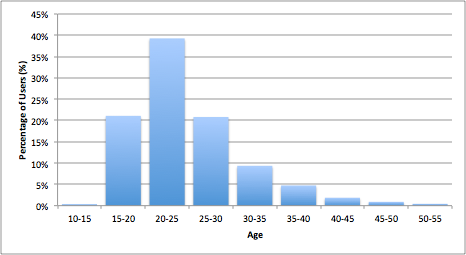
\includegraphics[width=9cm]{figures/age_breakdown}
    \caption{Age distribution of user profiles.}
    \label{fig:age_breakdown}
    \vspace{2em}
    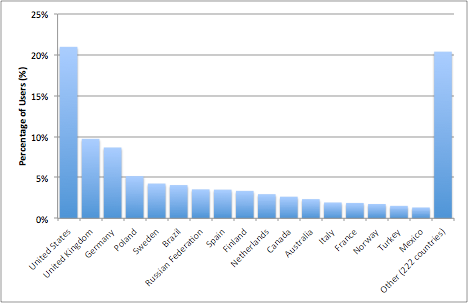
\includegraphics[width=9cm]{figures/country_breakdown}
    \caption{Country distribution of user profiles.}
    \label{fig:country_breakdown}
    \vspace{2em}
    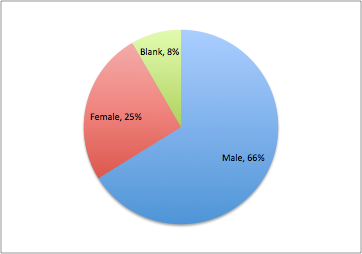
\includegraphics[width=9cm]{figures/gender_breakdown}
    \caption{Gender distribution of user profiles.}
    \label{fig:gender_breakdown}
\end{figure}

\clearpage

\section{Results}
The baseline that we began with was the Per-User Median script provided with the data. On Kaggle, this produced an error of 137.79, which we eventually discovered was quite good for the simplicity of the algorithm. We attempted to improve on this baseline using the following approaches, which increased complexity of the code in the hopes of improving the accuracy.

\subsection{Per-User-Artist-Cluster Median}
One thought we had after observing the workings of the Per-User Median approach was that the baseline could further be improved by simply identifying play medians on a per-user-per-genre basis instead of a per-user. Intuitively, if a user likes "Rock" artists and listens to "Rock" bands frequently, then a newly introduced "Rock" artist should have a higher likelihood of being played. In other words, two artists who are similar in genre should have similar play counts. \\

In order to execute this strategy, we first needed to cluster artists into different ``genres" or classes. To do so, we decided to use the Last.fm API to pull the most popular user-generated tags for each artists. These tags included musical genres, such as ``Rap", ``Rock", and ``Alternative." Once we had these tags, we used KMeans++ to cluster the artists into 50 classes based on binary indicators representing presence of certain tags.\\

From there, we created play medians for each cluster played by the user. In order to predict, we first found the cluster of the artist, then looked for the corresponding median of that cluster. If the user-cluster median did not exist (e.g., a user had previously never listened to a song of genre X), then we simply used the user-median play count in its place.\\

Unfortunately, this method produced a worse score on Kaggle of 164.6. We suspect that this approach did not work because of the lack of data on a user-cluster level. With small amounts of data (e.g., one song in a cluster), the median figure could be largely skewed by outliers, creating wildly incorrect predictions.

\subsection{KMeans}
We also tried KMeans clustering on the users to group similar types of users based on their profile data, which included age and country. We first generated a baseline K-means cross-validation score of 198.9 and subsequently tried to improve the score by feature extraction and model tuning. For instance, on a per-user level, we calculated a cluster ratio by which to scale up the user median. We further attempted to add age bucketing to better group users of similar age. Unfortunately, while these efforts did improve our score, they did not yield significant improvements to the KMeans output {\bf (Figure \ref{fig:kmeans_table})}.

 \begin{figure}[t]
    \centering
    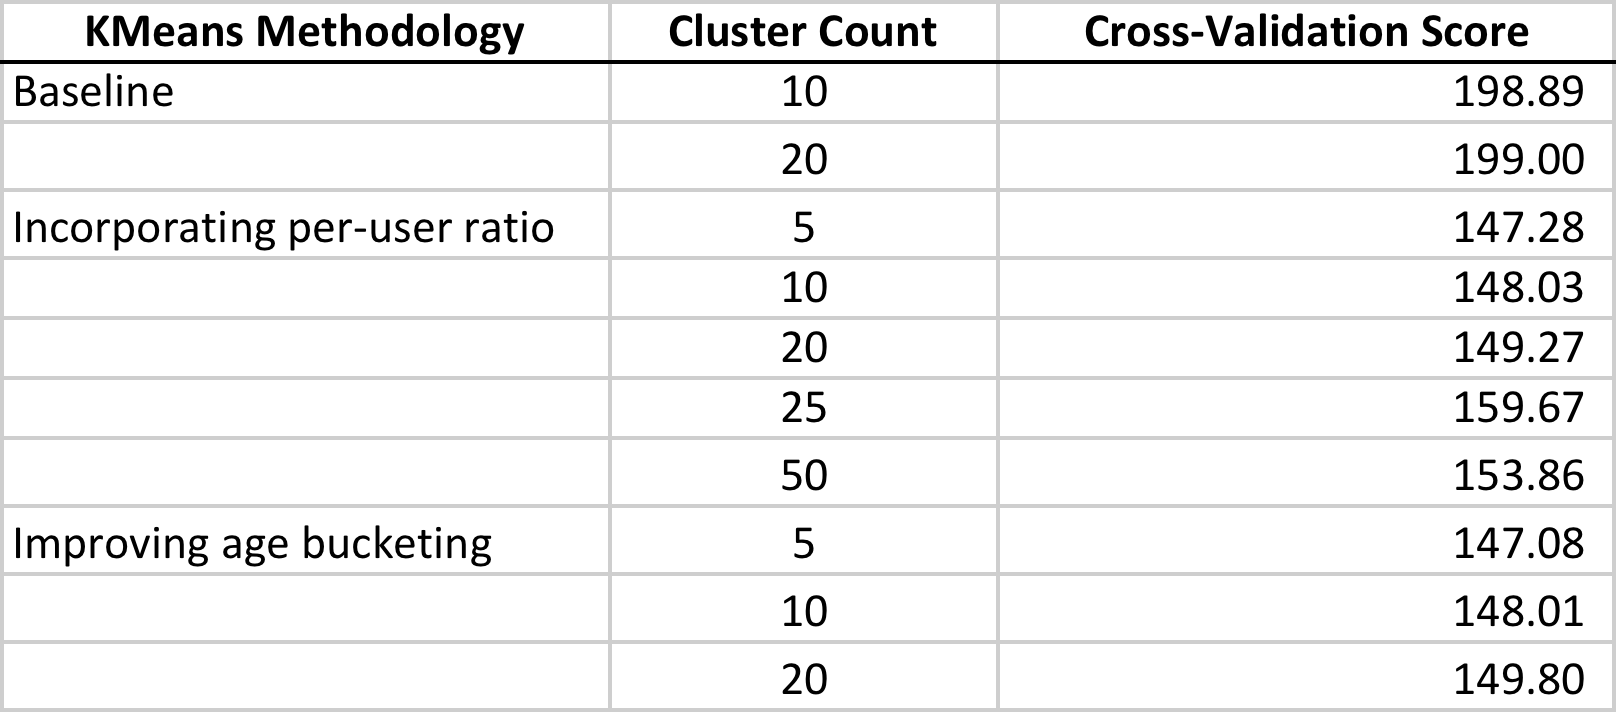
\includegraphics[width=12cm]{kmeans_table}
    \caption{KMeans data for various cluster sizes and .}
    \label{fig:kmeans_table}
\end{figure}


\subsection{Collaborative Filtering}
We also attempted to use Collaborative Filtering (CF) in order to improve our results. Collaborative Filtering is a technique that is commonly used in recommender systems. Essentially, CF uses similarity matrices in order to generate predictions. There are two-approaches to generating a similarity matrix: a user-based approach and an artist-based approach. In the user-based approach, if we are looking to understand how much a user X might play an artist Y, we first look for users that are similar to user X and then use their artist Y play counts to predict user X's play counts for artist Y. In the artist-based approach, we first look for artists that are similar to Y that user X has listened to previously and then use those play counts in order to predict user X's play counts for artist Y.\\

The problem that we ultimately encountered with CF was limited memory space. The user-artist matrix is a 233,286 $\times$ 2000 matrix. If we had more time, we might attempt to use machines with larger amounts of memory or Hadoop to divide the problem onto multiple machines. 

\subsection{Regression Clustering}
Another failed attempt consisted of combining both regression and clustering techniques. We began with the user data, and appended one column per artist. In each column, we filled the number of plays by that user for that artist if he/she had listened to them, and 0 otherwise. We then ran this entire table into a KMeans clustering algorithm to define a cluster to which each user belonged. From here, we switched to our user and artist table. We added a number of new features to this dataframe, including the user's cluster, the genre of the artist (which was a sort of true clustering), the median plays for that user, and the median plays on that artist. The idea was to allow the regression to center around the median values, and let the other features provide additional guidance to a more accurate value. \\

This method unfortunately suffered from the same issues that CF did. On numerous accounts, the machine would crash as it attempted to fit any sort of model to the aggregated data set we had generated due to the large size of the matrix.\\ 

\subsection{Co-occurrence}

Of all the methods that we attempted, the one that we found to work the best was building a co-occurrence matrix.  This matrix represented the probability of a user playing a song by a specific artist given that the user played songs by another artist.  We standardized these values by subtracting out the medians and dividing by the user's standard deviation.  We subtracted out the medians rather than the means since the means were very skewed, and the medians gave better predictions. \\

We also kept track of the number of times each set of artists occurred together in a user's data.  We then used these joint counts to normalize the co-occurrence matrix, in essence finding the mean co-occurrence across all users where co-occurrence existed. \\

For each user, for each artist, we calculated a weighted prediction using our normalized co-occurrence matrix.  We then multiplied this prediction by the user's standard deviation of plays and added back in the user's median, personalizing our prediction for this user and artist. This method worked the best of all the methods we tried giving us an error of 136.94 on Kaggle. \\

\section{Discussion}


 If we had more time, it would be interesting to attempt a mixture model on the data to see if that could significantly improve upon the baseline.  Also, we could attempt to run the Collaborative Filtering or the Regression Clustering on larger servers in the cloud.\\
 
 It was a little unsettling that our models could not clear the baseline by a significant amount. We had surmised that by including more information about the cluster to which the user-artist pair belonged, that the MAE would drop considerably, but the improvements were marginal. Predicting plays is a difficult task, and it was an added blow that half the techniques about which we were optimistic did not even work. \\ 
 
 We hypothesize that our models performed poorly due to three factors of the data: sparseness, skew, and outliers. On average, users listened to about 18 out of the 2000 artists, which meant finding common ground between users made it difficult to cluster users together from their similarities in listening. The data also suffered from a heavy skew; {\bf (Figure \ref{fig:skew})} demonstrates that the mean and median were far off, which means that the distribution of a user's plays were consistently right skewed, like a Poisson distribution. We observed that there were a few user-play pairs in the training set that were far beyond any median we calculated, and we hypothesized that there were similarly extreme outliers present in the test data as well. When predicting these values, we can be certain that our MAE will be appreciably affected by these outliers. 
 
 Overall, this was an interesting and challenging practical that proved the difficulty of creating individualized predictions based on a sparse data set.
 
 \begin{figure}[t]
    \centering
    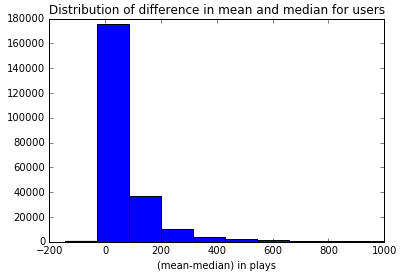
\includegraphics[width=9cm]{meanmedian}
    \caption{User medians were often left-skewed.}
    \label{fig:skew}
\end{figure}

 

\section {Code}
\begin{lstlisting}
#
# Github Repo:
# https://github.com/averyfaller/CS181Practical/tree/master/3
#


# coding: utf-8

# In[7]:

# Imports
import numpy as np
import csv
from sklearn import *

# Predict via the user-specific median.
# If the user has no data, use the global median.

# Hard-code file names
train_file = 'train.csv'
test_file  = 'test.csv'
soln_file  = 'predictions.csv'
profiles_file = 'profiles.csv'
artist_file = 'artists.csv'


# In[8]:

# Load the profile data.
profile_data = {}
user_ids = []

with open(profiles_file, 'r') as profile_fh:
    profile_csv = csv.reader(profile_fh, delimiter=',', quotechar='"')
    next(profile_csv, None)
    for row in profile_csv:
        # user,sex,age,country
        user    = row[0]
        sex     = row[1]
        age     = row[2]
        country = row[3]

        if age == '':
            age = -1
        if sex == '':
            sex = 'u'
    
        if not user in profile_data:
            profile_data[user] = {}
            user_ids.append(user)
        
        profile_data[user]['sex'] = sex
        profile_data[user]['age'] = int(age)
        profile_data[user]['country'] = country

print len(user_ids)


# In[9]:

print "Number of users in profiles: " + str(len(user_ids))
print ""
for user_id in user_ids[1:20]:
    print profile_data[user_id]


# In[10]:

# Create indicator variables
columns = ['i_MALE','i_FEMALE']

# Add countries
for user_id in user_ids:
    country = profile_data[user_id]['country']
    if country not in columns:
        columns.append(country)

# Add ages
ages = [15, 20, 25, 30, 35, 40, 45, 50, 55, 10000] # AGES
columns.extend(ages)
    
# Construct matrix
profile_matrix = np.zeros((len(user_ids), len(columns)))
age_matrix = np.zeros((len(user_ids), len(ages)))
for i, user_id in enumerate(user_ids):
    profile = profile_data[user_id]

    # Create indicator variable for MALE
    if profile['sex'] == 'm':
        profile_matrix[i, 0] = 1
    # Create indicator variable for FEMALE    
    elif profile['sex'] == 'f':
        profile_matrix[i, 1] = 1
        
    # Add a 1 for the country indicator
    country = profile['country']
    country_col = columns.index(country)
    profile_matrix[i, country_col] = 1

    # TODO: Calculate median age, replace nulls with 
    
    # Add age
    index = 0
    for j, age in enumerate(ages):
        if profile['age'] < age:
            index = j
        else:
            break
    age_matrix[i, index] = 1
    
profile_matrix = np.hstack((profile_matrix, age_matrix))


# In[11]:

# Examine the data
profile_matrix.shape
profile_matrix[1:10]


# In[12]:

user_pos_by_id = {}
for i, user_id in enumerate(user_ids):
    user_pos_by_id[user_id] = i


# In[13]:

# Load the artist data.
artist_names = {}
artist_ids = []

with open(artist_file, 'r') as artist_fh:
    artist_csv = csv.reader(artist_fh, delimiter=',', quotechar='"')
    next(artist_csv, None)
    for row in artist_csv:
        # user,sex,age,country
        artist    = row[0]
        name      = row[1]
        
        artist_names[artist] = name
        artist_ids.append(artist)
        
artist_pos_by_id = {}
for i, artist_id in enumerate(artist_ids):
    artist_pos_by_id[artist_id] = i


# In[14]:

# Load the training data.
train_data = {}
train_user_ids = []

# TRAIN-TEST SPLIT FOR TESTING PURPOSES
# Need to split on a per-user-artist level, not just per-user level
train_train_data = {}
train_test_data = {}

with open(train_file, 'r') as train_fh:
    train_csv = csv.reader(train_fh, delimiter=',', quotechar='"')
    next(train_csv, None)
    for row in train_csv:
        user   = row[0]
        artist = row[1]
        plays  = row[2]
    
        if not user in train_data:
            train_data[user] = {}
            train_user_ids.append(user)
        
        train_data[user][artist] = int(plays)
        
        # Build train and test split
        if np.random.uniform(0,1,1) < .75:
            if not user in train_train_data:
                train_train_data[user] = {}
            train_train_data[user][artist] = int(plays)
        else:
            if not user in train_test_data:
                train_test_data[user] = {}
            train_test_data[user][artist] = int(plays)


# In[8]:

# Examine the data
print "Number of users in train: " + str(len(train_user_ids))
print ""
for user_id in train_user_ids[1:3]:
    print train_data[user_id]


# In[15]:

# CALCULATE THE NUMBER OF SONGS WE ARE ESTIMATING IN OUR TRIAN_TEST SAMPLE
num_songs_estimating = 0

for user, user_data in train_test_data.iteritems():
    for artist, plays in user_data.iteritems():
        num_songs_estimating += 1
        
print num_songs_estimating


# ## KMeans - Let's Cluster the Users

# In[114]:

KM = sklearn.cluster.KMeans(n_clusters=5, init='k-means++', n_init=10, max_iter=300, tol=0.0001, precompute_distances='auto', verbose=0, random_state=37)
# Calls fit and then predict
predict = KM.fit_predict(profile_matrix)


# In[115]:

print "The objective function: %f" % KM.score(profile_matrix) 


# In[109]:

# Examine the predicted clusters
print predict[1:10]


# ## Keep track of score
# 
# ### Indicators for basic params
# 5 clusters: -4578883.573153
# 10 clusters: -948858.492895
# 20 clusters: -448359.382828
# 25 clusters:  -372704.076086
# 
# ### Better indicator columns for age:
# 5 clusters: -211766.969515
# 10 clusters: -170864.058997
# 20 clusters: -129169.230617

# ## Global and User Medians (Given) with KMeans Modifications

# In[134]:

abs_error = 0

# Compute the global median and per-user median.
plays_array  = []
user_medians = {}
artist_plays_array = {}

drop_ratio = .9

cluster_plays_array = {}

for user, user_data in train_train_data.iteritems():
    user_plays = []
    cluster_id = predict[user_pos_by_id[user]]
    if cluster_id not in cluster_plays_array:
        cluster_plays_array[cluster_id] = []
    
    for artist, plays in user_data.iteritems():
        plays_array.append(plays)
        user_plays.append(plays)
        
        if artist not in artist_plays_array:
            artist_plays_array[artist] = []
        
        artist_plays_array[artist].append(plays)
        
    user_median = np.median(np.array(user_plays))
    user_medians[user] = user_median
    cluster_plays_array[cluster_id].append(user_median)
    
global_median = np.median(np.array(plays_array))
#global_mean = np.mean(np.array(plays_array))

cluster_ratios = {}
for cluster_id, cluster_data in cluster_plays_array.iteritems():
    cluster_ratios[cluster_id] = np.median(cluster_data) / global_median

artist_ratios = {}
for artist, artist_data in artist_plays_array.iteritems():
    #artist_ratios[artist] = np.median(artist_data) - global_median
    artist_ratios[artist] = np.median(artist_data) / global_median
    
for user, user_data in train_test_data.iteritems():
    cluster_id = predict[user_pos_by_id[user]]
    for artist, plays in user_data.iteritems():
        if user in user_medians:
            prediction = user_medians[user] * artist_ratios[artist] * drop_ratio * cluster_ratios[cluster_id]
            abs_error += abs(prediction - plays) 
        else:
            print "User", user, "not in train_train data."
            abs_error += abs(global_median - plays)
            
print "MEAN ABSOLUTE ERROR %f" % (abs_error / num_songs_estimating)


# ## Co-Occurance

# In[16]:

# Construct the co-occurance matrix
artist_plays_cooccurance = np.zeros((len(artist_pos_by_id), len(artist_pos_by_id)))

for user, user_data in train_train_data.iteritems():
    for artist_1, plays_1 in user_data.iteritems():
        for artist_2, plays_2 in user_data.iteritems():
            artist_plays_cooccurance[artist_pos_by_id[artist_1], artist_pos_by_id[artist_2]] += plays_2 * 1.0 / plays_1


# In[17]:

# Normalize!
for i in range(len(artist_pos_by_id)):
    norm_factor = artist_plays_cooccurance[i, i]
    for j in range(len(artist_pos_by_id)):
        artist_plays_cooccurance[i, j] /= norm_factor


# In[18]:

print artist_plays_cooccurance[0:10,0:10]


# In[22]:

abs_error = 0

plays_array  = []
user_medians = {}
user_total_plays = {}
artist_plays_array = {}

drop_ratio = 1.0

cluster_plays_array = {}

for user, user_data in train_train_data.iteritems():
    user_plays = []
    #cluster_id = predict[user_pos_by_id[user]]
    #if cluster_id not in cluster_plays_array:
    #    cluster_plays_array[cluster_id] = []
    
    for artist, plays in user_data.iteritems():
        plays_array.append(plays)
        user_plays.append(plays)
        
        if artist not in artist_plays_array:
            artist_plays_array[artist] = []
        
        artist_plays_array[artist].append(plays)
        
    user_median = np.median(np.array(user_plays))
    user_medians[user] = user_median
    user_total_plays[user] = np.sum(user_plays)
#    cluster_plays_array[cluster_id].append(user_median)
    
global_median = np.median(np.array(plays_array))
#global_mean = np.mean(np.array(plays_array))

#cluster_ratios = {}
#for cluster_id, cluster_data in cluster_plays_array.iteritems():
#    cluster_ratios[cluster_id] = np.median(cluster_data) / global_median

artist_ratios = {}
for artist, artist_data in artist_plays_array.iteritems():
    #artist_ratios[artist] = np.median(artist_data) - global_median
    artist_ratios[artist] = np.median(artist_data) / global_median
    
itr = 0
    
# PREDICT!
for user, user_data in train_test_data.iteritems():
    itr += 1
    
    #cluster_id = predict[user_pos_by_id[user]]
    if user in user_total_plays:
        user_total = user_total_plays[user]
        user_train = train_train_data[user]
    
        for artist_to_predict, plays_to_predict in user_data.iteritems():
            prediction = 0
            for artist_cooccur, plays_cooccur in user_train.iteritems():
                prediction += (1.0 * plays_cooccur / user_total) * (plays_cooccur * artist_plays_cooccurance[artist_pos_by_id[artist_cooccur], artist_pos_by_id[artist_to_predict]])
        
            #prediction = user_medians[user] * artist_ratios[artist] * drop_ratio * cluster_ratios[cluster_id]
            abs_error += abs(prediction - plays_to_predict) 
            if itr < 10:
                print "User", user, "Actual: ", plays_to_predict, "Prediction: ", prediction

    else:
        print "User", user, "not in train_train data."
        for artist_to_predict, plays_to_predict in user_data.iteritems():
            abs_error += abs(global_median - plays_to_predict)
            
print "MEAN ABSOLUTE ERROR %f" % (abs_error / num_songs_estimating)


# In[57]:

# Construct the co-occurance matrix
artist_plays_cooccurance = np.zeros((len(artist_pos_by_id), len(artist_pos_by_id)))

for user, user_data in train_train_data.iteritems():
    for i, (artist_1, plays_1) in enumerate(user_data.iteritems()):
        for j, (artist_2, plays_2) in enumerate(user_data.iteritems()):
            if j > i:
                artist_plays_cooccurance[artist_pos_by_id[artist_1], artist_pos_by_id[artist_2]] += plays_2 / plays_1
                artist_plays_cooccurance[artist_pos_by_id[artist_2], artist_pos_by_id[artist_1]] += plays_1 / plays_2
            elif j==i:
                artist_plays_cooccurance[artist_pos_by_id[artist_1], artist_pos_by_id[artist_1]] += 1
            
# Normalize!
for i in range(len(artist_pos_by_id)):
    norm_factor = artist_plays_cooccurance[i, i]
    for j in range(len(artist_pos_by_id)):
        artist_plays_cooccurance[i, j] /= norm_factor

itr = 0
abs_error = 0
    
# PREDICT!
for user, user_data in train_test_data.iteritems():
    itr += 1
    
    #cluster_id = predict[user_pos_by_id[user]]
    if user in user_total_plays:
        user_total = user_total_plays[user]
        user_train = train_train_data[user]
        if itr < 10:
            print "------"
            print "User", user, "TRAIN: ", user_train
    
        for artist_to_predict, plays_to_predict in user_data.iteritems():
#            prediction = []
            prediction = 0
            for artist_cooccur, plays_cooccur in user_train.iteritems():
                #if plays_cooccur > 1:
                    #prediction.append(plays_cooccur * artist_plays_cooccurance[artist_pos_by_id[artist_cooccur], artist_pos_by_id[artist_to_predict]])
                prediction += 1.0*plays_cooccur/user_total * (plays_cooccur * artist_plays_cooccurance[artist_pos_by_id[artist_cooccur], artist_pos_by_id[artist_to_predict]])
        
            #if len(prediction) > 0:
            #    prediction = np.mean(prediction)#1.0 * prediction / user_total
            #else:
            #    prediction = 1.0
            w_prediction = user_medians[user] * .9 + prediction * .4
            #prediction = prediction# * user_medians[user]* artist_ratios[artist]
            #user_medians[user] * artist_ratios[artist] * drop_ratio * cluster_ratios[cluster_id]
            abs_error += abs(w_prediction - plays_to_predict) 
            if itr < 10:
                print "Actual: ", plays_to_predict, "Prediction: ", w_prediction, (prediction > plays_to_predict), "predict: ", prediction

    else:
        print "User", user, "not in train_train data."
        for artist_to_predict, plays_to_predict in user_data.iteritems():
            abs_error += abs(global_median - plays_to_predict)
            
print "MEAN ABSOLUTE ERROR %f" % (abs_error / num_songs_estimating)


# ### Co-occurance by ratio to user median

# In[74]:

abs_error = 0

plays_array  = []
user_medians = {}
user_means = {}
user_total_plays = {}
user_stds = {}
artist_plays_array = {}

drop_ratio = 1.0

cluster_plays_array = {}

for user, user_data in train_train_data.iteritems():
    user_plays = []
    #cluster_id = predict[user_pos_by_id[user]]
    #if cluster_id not in cluster_plays_array:
    #    cluster_plays_array[cluster_id] = []
    
    for artist, plays in user_data.iteritems():
        plays_array.append(plays)
        user_plays.append(plays)
        
        if artist not in artist_plays_array:
            artist_plays_array[artist] = []
        
        artist_plays_array[artist].append(plays)
        
    user_median = np.median(np.array(user_plays))
    user_medians[user] = user_median
    user_means[user] = np.mean(user_plays)
    user_stds[user] = np.std(user_plays)
    user_total_plays[user] = np.sum(user_plays)


# In[77]:

# Construct the co-occurance matrix
artist_plays_cooccurance = np.zeros((len(artist_pos_by_id), len(artist_pos_by_id)))

for user, user_data in train_train_data.iteritems():
    user_median = user_medians[user]
    user_mean = user_means[user]
    user_std = user_stds[user]
    if user_std == 0:
        user_std = 1.0
    for i, (artist_1, plays_1) in enumerate(user_data.iteritems()):
        for j, (artist_2, plays_2) in enumerate(user_data.iteritems()):
            if j > i:
                artist_plays_cooccurance[artist_pos_by_id[artist_1], artist_pos_by_id[artist_2]] += (1.0 * plays_2 - user_median) / user_std
                artist_plays_cooccurance[artist_pos_by_id[artist_2], artist_pos_by_id[artist_1]] += (1.0 * plays_1 - user_median) / user_std
            elif j==i:
                artist_plays_cooccurance[artist_pos_by_id[artist_1], artist_pos_by_id[artist_1]] += 1#(1.0 * plays_1 - user_mean) / user_mean
            
# Normalize!
for i in range(len(artist_pos_by_id)):
    norm_factor = artist_plays_cooccurance[i, i]
    for j in range(len(artist_pos_by_id)):
        artist_plays_cooccurance[i, j] /= norm_factor


# In[78]:

itr = 0
abs_error = 0
    
# PREDICT!
for user, user_data in train_test_data.iteritems():
    itr += 1
    
    #cluster_id = predict[user_pos_by_id[user]]
    if user in user_total_plays:
        user_total = user_total_plays[user]
        user_train = train_train_data[user]
        if itr < 10:
            print "------"
            print "User", user, "TRAIN: ", user_train
    
        for artist_to_predict, plays_to_predict in user_data.iteritems():
#            prediction = []
            prediction = 0
            for artist_cooccur, plays_cooccur in user_train.iteritems():
                #if plays_cooccur > 1:
                    #prediction.append(plays_cooccur * artist_plays_cooccurance[artist_pos_by_id[artist_cooccur], artist_pos_by_id[artist_to_predict]])
                prediction += (plays_cooccur * artist_plays_cooccurance[artist_pos_by_id[artist_cooccur], artist_pos_by_id[artist_to_predict]])
        
            prediction = prediction / user_total
        
            #if len(prediction) > 0:
            #    prediction = np.mean(prediction)#1.0 * prediction / user_total
            #else:
            #    prediction = 1.0
            user_std = user_stds[user]
            if user_std == 0:
                user_std = 1.0
            w_prediction = user_medians[user] + user_std * prediction #* user_medians[user] #user_medians[user] * .9 + prediction * .4
            #prediction = prediction# * user_medians[user]* artist_ratios[artist]
            #user_medians[user] * artist_ratios[artist] * drop_ratio * cluster_ratios[cluster_id]
            abs_error += abs(w_prediction - plays_to_predict) 
            if itr < 10:
                print "Actual: ", plays_to_predict, "Prediction: ", w_prediction, ", Mean: ", user_means[user], "predict: ", prediction, user_means[user] * prediction

    else:
        print "User", user, "not in train_train data."
        for artist_to_predict, plays_to_predict in user_data.iteritems():
            abs_error += abs(global_median - plays_to_predict)
            
print "MEAN ABSOLUTE ERROR %f" % (abs_error / num_songs_estimating)


# ### KMEANS CLUSTERING

# In[81]:

abs_error = 0

cluster_artist_plays = {}

for user, user_data in train_train_data.iteritems():
    cluster_id = predict[user_pos_by_id[user]]
    for artist, plays in user_data.iteritems():
        if cluster_id not in cluster_artist_plays:
            cluster_artist_plays[cluster_id] = {}
        
        if artist not in cluster_artist_plays[cluster_id]:
            cluster_artist_plays[cluster_id][artist] = []
        
        cluster_artist_plays[cluster_id][artist].append(plays)

print "Finished setting up cluster author play dictionary, running test now"

# Precalculate the cluster-artist medians
cluster_artist_medians = {}
for cluster_id, cluster_data in cluster_artist_plays.iteritems():
    artist_medians = {}
    for artist, plays in cluster_data.iteritems():
        artist_medians[artist] = np.median(plays)
    cluster_artist_medians[cluster_id] = artist_medians

for user, user_data in train_test_data.iteritems():
    for artist, plays in user_data.iteritems():
        cluster_id = predict[user_pos_by_id[user]]
        
        if artist in cluster_artist_plays[cluster_id]:
            abs_error += abs(np.median(cluster_artist_plays[cluster_id][artist]) - plays)
        elif user in user_medians:
            abs_error += abs(user_medians[user] - plays)
        else:
            print "User", user, "not in train_train data."
            abs_error += abs(global_median - plays)
            #print "Cluster+Artist: ", cluster_id, artist, "not in train_train data."
            #abs_error += abs(0 - plays)
            
print "MEAN ABSOLUTE ERROR %f" % (abs_error / num_songs_estimating)


# In[123]:

abs_error = 0

cluster_artist_plays = {}

# The median number of per user per cluster
cluster_user_plays = {}

# The cluster medians
cluster_medians = {}

user_medians = {}

drop_ratio = .8

for user, user_data in train_train_data.iteritems():
    cluster_id = predict[user_pos_by_id[user]]
    user_plays = []
    for artist, plays in user_data.iteritems():
        if cluster_id not in cluster_artist_plays:
            cluster_artist_plays[cluster_id] = {}
        
        if artist not in cluster_artist_plays[cluster_id]:
            cluster_artist_plays[cluster_id][artist] = []
        
        cluster_artist_plays[cluster_id][artist].append(plays)

        user_plays.append(plays)

    median = np.median(np.array(user_plays))
    user_medians[user] = median
    if cluster_id not in cluster_user_plays:
        cluster_user_plays[cluster_id] = []
    cluster_user_plays[cluster_id].append(median) 
    
# Calculate per-cluster user median
for cluster_id, user_plays in cluster_user_plays.iteritems():
    cluster_medians[cluster_id] = np.median(user_plays)
    
user_ratios = {}
    
# Calculate the user-cluster play ratios
for user_id, median_plays in user_medians.iteritems():
    cluster_id = predict[user_pos_by_id[user_id]]
    user_ratios[user_id] = 1.0 * median_plays / cluster_medians[cluster_id]
        
print "Finished setting up cluster author play dictionary, running test now"

# Precalculate the cluster-artist medians
cluster_artist_medians = {}
for cluster_id, cluster_data in cluster_artist_plays.iteritems():
    artist_medians = {}
    for artist, plays in cluster_data.iteritems():
        artist_medians[artist] = np.median(plays)
    cluster_artist_medians[cluster_id] = artist_medians

# PREDICT!
for user, user_data in train_test_data.iteritems():
    for artist, plays in user_data.iteritems():
        cluster_id = predict[user_pos_by_id[user]]
        if artist in cluster_artist_plays[cluster_id]:
            user_ratio = 1.0
            if user in user_ratios:
                user_ratio = user_ratios[user]
            prediction = user_ratio * cluster_artist_medians[cluster_id][artist] * drop_ratio
            abs_error += abs(prediction - plays)
        elif user in user_medians:
            abs_error += abs(user_medians[user] - plays)
        else:
            print "User", user, "not in train_train data."
            abs_error += abs(global_median - plays)
            
print "MEAN ABSOLUTE ERROR %f" % (abs_error / num_songs_estimating)

# ## OUTPUT

# In[30]:

# Compute the global median and per-user median.
plays_array  = []
user_medians = {}
for user, user_data in train_data.iteritems():
    user_plays = []
    for artist, plays in user_data.iteritems():
        plays_array.append(plays)
        user_plays.append(plays)

    user_medians[user] = np.median(np.array(user_plays))
global_median = np.median(np.array(plays_array))

# Write out test solutions.
with open(test_file, 'r') as test_fh:
    test_csv = csv.reader(test_fh, delimiter=',', quotechar='"')
    next(test_csv, None)

    with open(soln_file, 'w') as soln_fh:
        soln_csv = csv.writer(soln_fh,
                              delimiter=',',
                              quotechar='"',
                              quoting=csv.QUOTE_MINIMAL)
        soln_csv.writerow(['Id', 'plays'])

        for row in test_csv:
            id     = row[0]
            user   = row[1]
            artist = row[2]

            if user in user_medians:
                soln_csv.writerow([id, user_medians[user]])
            else:
                print "User", id, "not in training data."
                soln_csv.writerow([id, global_median])
                

\end{lstlisting}
\end{document}
